\section{Special materials}
\subsection{Rigid Material}  This model was designed for use with the
\Textsfc{specified contact} model described in Section~\ref{Sec:Contact}.
It is designed to compute zero stress and identity deformation of the material,
and is basically a fast place-holder for materials that should not develop
any stress.

\begin{lstlisting}[language=XML]
  <constitutive_model type="rigid">
  </constitutive_model>
\end{lstlisting}

\begin{minipage}[t]{0.9\textwidth}
  \centering
  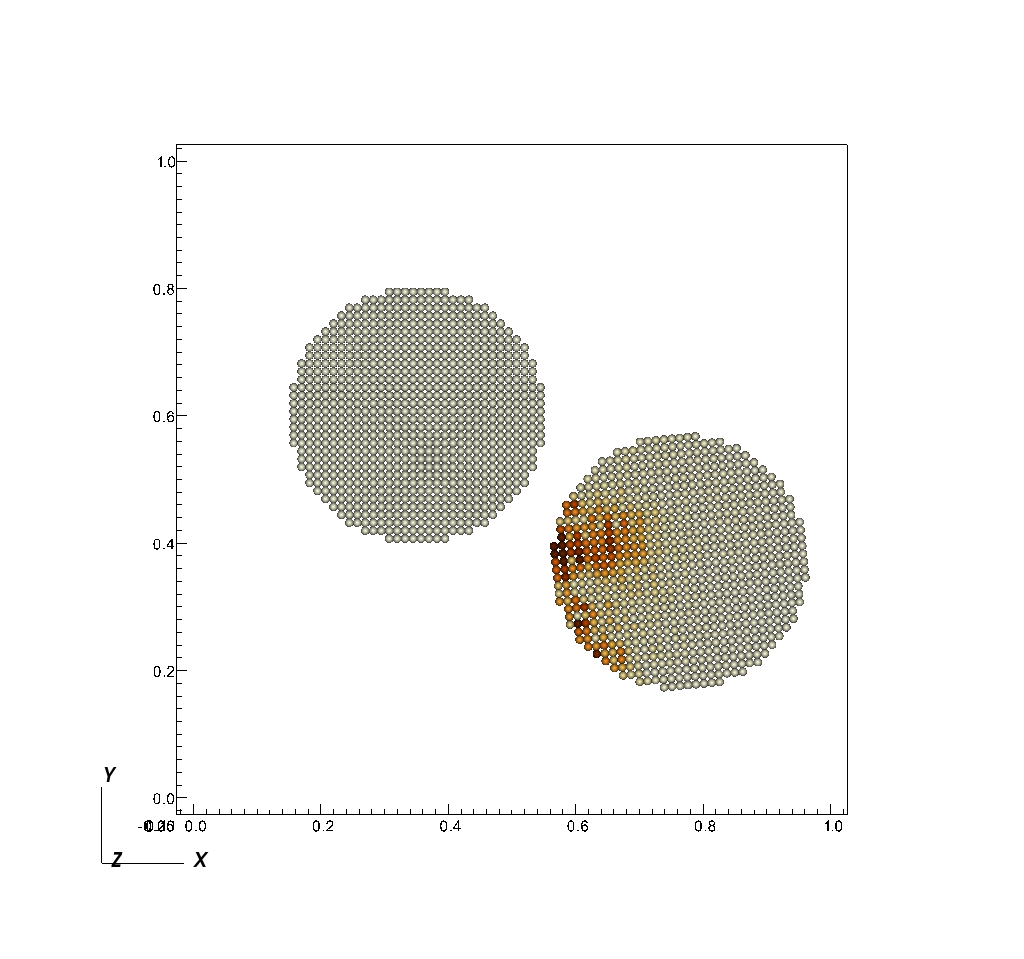
\includegraphics[width=0.5\columnwidth]{FIGS/contact/specified2.png}
  \captionof{figure}{A \Textsfc{rigid} disk (left) interacting with a deformable disk (right).}
\end{minipage}

\subsection{Ideal Gas}  
The ideal gas material provides an equation of state capability that allows
compression but no shear or tension.  Usage is:
\begin{lstlisting}[language=XML]
  <constitutive_model type="ideal_gas">
    <gamma> 1.4 </gamma>
    <specific_heat> 800.0 </specific_heat>
    <reference_pressure> 101325.0 </reference_pressure>
  </constitutive_model>
\end{lstlisting}


\subsection{Water}  This is a model for water, reported in \cite{water_model_ref}.
The P-V relationship is given by:
\begin{equation}
p=\kappa\left[\left(\frac{\rho}{\rho_0}\right)^{\gamma} - 1\right]
\end{equation}
Shear stress is simple Newtonian behavior.  It has not been validated,
but gives qualitatively reasonable behavior.  Usage is given by:
\begin{lstlisting}[language=XML]
              <constitutive_model type="water">
                 <bulk_modulus>15000.0</bulk_modulus>
                 <viscosity>.5</viscosity>
                 <gamma>7.0</gamma>
               </constitutive_model>
\end{lstlisting}
